%! TEX root = report1_week2.tex
\documentclass[11pt,a4paper]{article}

% --- Essential Packages ---
\usepackage[utf8]{inputenc}
\usepackage[margin=1in]{geometry}
\usepackage{hyperref}
\usepackage{amsmath,amssymb}
\usepackage{graphicx}
\usepackage{booktabs}
\usepackage{titlesec}
\usepackage{titletoc}
\usepackage{listings}
\usepackage{xcolor}
\usepackage{float}

% --- Section Formatting (No Numbering for \section) ---
\titleformat{\section}{\normalfont\Large\bfseries}{}{0pt}{}

\titlecontents{section}
  [0pt]
  {\addvspace{1.2em}\bfseries}
  {}
  {}
  {\hfill\contentspage}

% --- Hyperref Setup ---
\hypersetup{
    colorlinks=true,
    linkcolor=black,        % Internal links (Table of Contents, references) stay black
    filecolor=magenta,      
    urlcolor=blue,          % Web URLs
    citecolor=black         % Citations stay black
}

% --- Code Listing Setup ---
\lstset{
    basicstyle=\ttfamily\small,
    numbers=left,
    numberstyle=\tiny,
    stepnumber=1,
    numbersep=5pt,
    tabsize=4,
    showstringspaces=false,
    breaklines=true,
    frame=single
}

% --- Document Information ---
\title{\textbf{COS40003: Concurrent Programming} \\ \Large Report 1: Learning Summary (Weeks 1--2)}
\author{Dang Duc Minh \\[0.3em]     Student ID: 105559691}
\date{}

\begin{document}

\maketitle  
\tableofcontents
\newpage

% ==============================================================================
% SECTION: WEEK 1 - INTRODUCTION TO CONCURRENT PROGRAMMING
% ==============================================================================
\section{Week 1 - Introduction}

\subsection{Concurrent Computing}
% Perspective (observer's view), time-sharing, concurrency control
\textbf{Concurrent computing} is a fundamental computing paradigm that means multiple computational 
tasks are being executed on a same time period, but not necessarily 
simultaneously. Instead of processing tasks sequentially, the OS (operating system) will manages 
several execution flows at once to maximize resource utilization.

\hspace{5pt}

\noindent Concurrent computing relies heavily on \textbf{time-sharing}. The OS divides 
the CPU into small execution flows and rapidly switches between active processes. This approach
fundamentally maximizes system effciency by allowing processes that are ready to be executed to be
processed continously.

\hspace{5pt}

\noindent Coordinating concurrent tasks requires addresing two fundamental challanges:
 

\begin{enumerate}
    \item \textbf{Scheduling:} Determining which process executes next to ensure fairness and response time.
    \item \textbf{Concurrency Control:} Managing shared resources to prevent \textbf{race conditions} (inconsistent data or state caused by timing issues) and \textbf{deadlocks} (processes that wait indefinitely where two or more threads or processes wait indefinitely for each other, which prevents any of them from making progress).
\end{enumerate}

\noindent A common example of concurrent computing is a web browser (e.g., Chrome, Safari)
is opening multiple tabs at one, where each tab are doing seperate tasks such as playing a video, downloading a file,
or fetching live chat messages.

\hspace{5pt}

\noindent According to Rob Pike, co-creator of the Go programming language: 
\textbf{``concurrency is about dealing with lots of things at once, while parallelism is about doing lots of things at once''}~\cite{pike2012}.



\subsection{Parallel Computing}
% Perspective (system's view), hardware parallelism, subtask decomposition
\textbf{Parallel computing} is a computing architecture in which multiple calculations or execution flows
are carried out at the exact same time. Concurrent computing often creates an illusion of 
simultaneous progress on a single CPU from the user's perspective. Parallelism, on the other hand, represents multiple executions at the exact same time, as illustrated in Figure~\ref{fig:concurrent_vs_parallel}.

\begin{figure}[htbp]
    \centering
    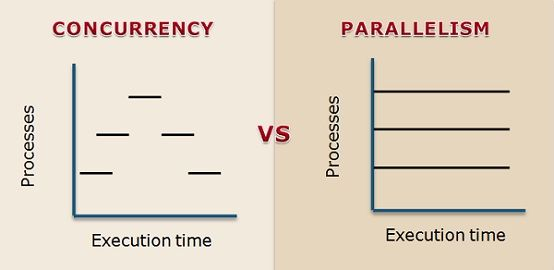
\includegraphics[width=0.55\textwidth]{report1_images/parallel1.jpg}
    \caption{Concurrent execution vs. Parallel execution~\cite{techdifferences_concurrency_parallelism}.}
    \label{fig:concurrent_vs_parallel}
\end{figure}

\hspace{5pt}

\noindent In parallel computing, a large computational workload is broken down into smaller, independent subtasks that can be executed concurrently.
Each subtasks are executed simultaneously on seperate processors, and once they are finished, the individual sub-results are merged to produce the final
output. In a typical parallel computing architectures, processors communicate directly through \textbf{shared memory} to ensure
low-latency data exchange across processes.

\hspace{5pt}

\noindent A real-world example of parallel computing is a \textbf{Graphics Processing Unit (GPU)}, which 
comprises thousands of smaller arithmetic cores for executing identical operations such as rendering graphics or computing matrix multiplications
using the \textbf{Single Instruction, Multiple Data (SIMD) architecture} (shown in Figure~\ref{fig:simd}).

\begin{figure}[htbp]
    \centering
    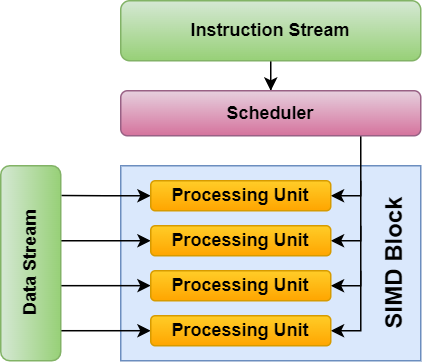
\includegraphics[width=0.43\textwidth]{report1_images/parallel2.png}
    \caption{SIMD Architecture~\cite{rastergrid_simd_gpu}.}
    \label{fig:simd}
\end{figure}



\subsection{Distributed Computing}
% Autonomous nodes, private memory, message passing
Distributed computing consists of multiple autonomous computing entities that are connected through a shared network to solve complex computational problems.
A fundamental architectural distinction between parallel computing and distributed computing lies in memory organization. 
In parallel computing, processors shares a common memory space to exchange information directly. But for distributed computing, each individual computer cannot access each other's memory directly and must exchange information through \textbf{message passing} (communication protocols or middleware)~\cite{gfg_distributed_system}    (shown in Figure~\ref{fig:distributed_sys}).

\begin{figure}[htbp]
    \centering
    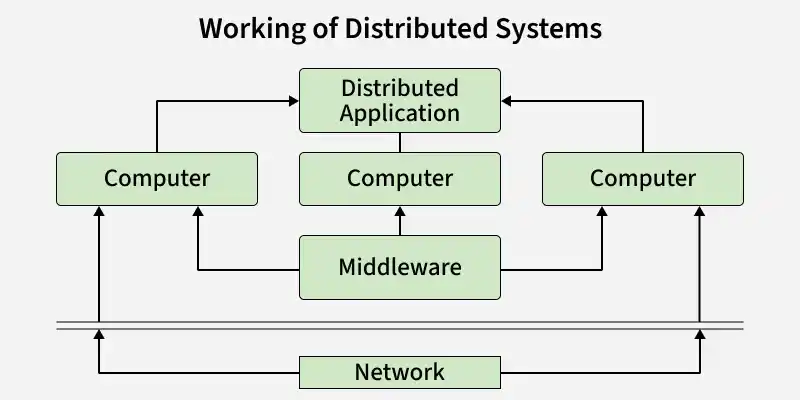
\includegraphics[width=0.55\textwidth]{report1_images/distributed1.png}
    \caption{Architecture of a Distributed System~\cite{gfg_distributed_system}.}
    \label{fig:distributed_sys}
\end{figure}

\hspace{5pt}

\noindent Distributed computing architectures are commonly classified into two primary paradigms:

\begin{enumerate}
    \item \textbf{Cluster computing:} Composed of \textbf{homogeneous} machines, which feature similar hardware configurations and identical OSs, that are \textbf{co-located} within a single area. This architecture is designed for high availability and high-performance computing.
    \item \textbf{Grid computing:}  Comprised of \textbf{heterogeneous} computing entities that are \textbf{geographically dispersed} across different physical locations. Grid computing represents the conceptual predecessor to modern cloud infrastructure.
\end{enumerate}

\noindent A real-world example that implements both cluster and grid computing is the \textbf{Worldwide LHC Computing Grid (WLCG)}~\cite{cern_wlcg}. Local server
clusters are deployed for high-performance batch processing, and these clusters are linked globally into a centralized grid to analyze high volumes of data.

\subsection{Cloud Computing}
% Service abstraction (IaaS, PaaS, SaaS), distributed backend infrastructure

\textbf{Cloud Computing} is one of the most demanded computational infrastruture in modern computing, delivering services such as servers, storage, databases, and networking over the Internet. 

\hspace{5pt}

\noindent The fundamental goal of cloud computing is abstraction, which hides the underlying physical hardware and maintenance complexity from users, allowing them to access on demand resources with seamless scalability and minimal configuration. Behind this abstraction, cloud computing relies extensively on
distributed systems since it coordinates massive networks of server clusters to ensure high availability and data redundancy across multiple regions.

\hspace{5pt}

\noindent Cloud services are organized into three primary architectural models:

\begin{enumerate}
    \item \textbf{Infrastructure as a Service (IaaS):} Provides virtualized computing infrastructure, including virtual machines, block storage, and virtual networks (e.g., AWS EC2, Microsoft Azure VMs)
    \item \textbf{Platform as a Service (PaaS):} Provides a managed execution environment and development framework where developers can build and run applications without configuring the underlying OS or runtime (e.g., Vercel, Firebase)
    \item \textbf{Software as a Service (SaaS):} Provides software applications that can be directly accessed via web browsers (e.g., Microsoft 365, Google Docs).
\end{enumerate}

\begin{figure}[H]
    \centering
    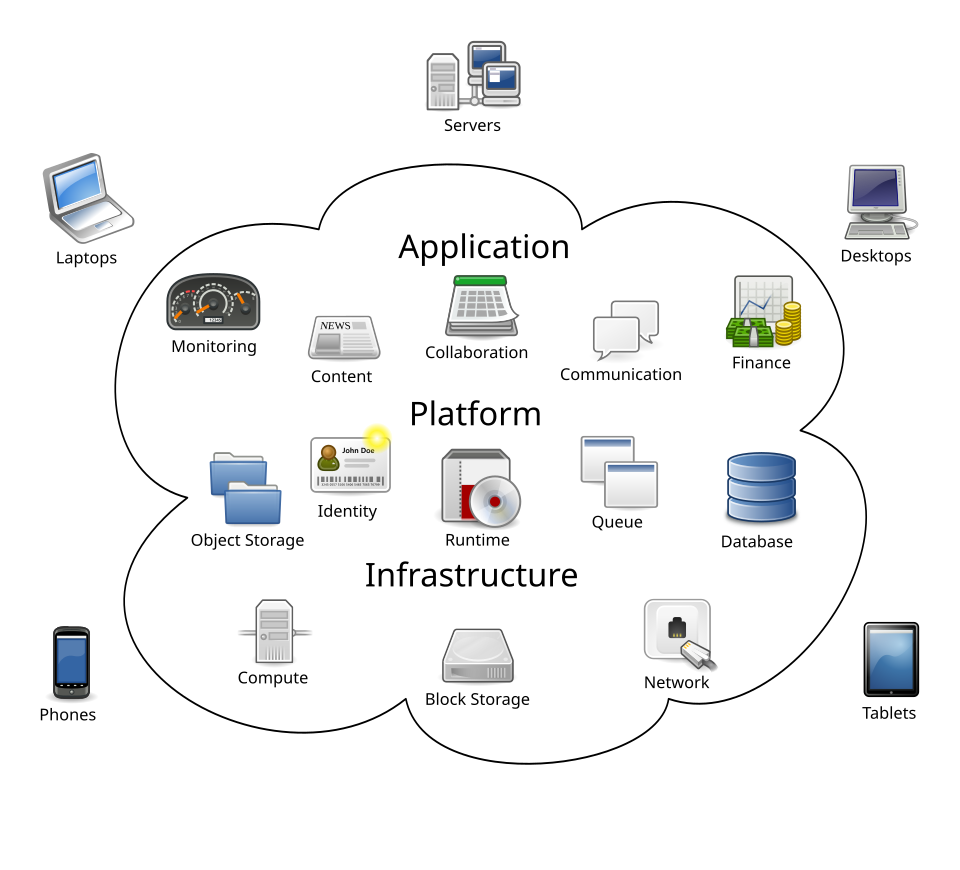
\includegraphics[width=0.48\textwidth]{report1_images/cloud1.png}
    \caption{Cloud Computing Logical Architecture and Service Models~\cite{wiki_cloud_computing}.}
    \label{fig:cloud_computing}
\end{figure}

\subsection{Fog and Edge Computing}
% Proximity to data-generating devices, IoT applications, latency reduction

\textbf{Fog and Edge computing} designed to bring processing and data storage closer to data-generating sources, primarily Internet of Things (IoT) devices. These computing paradigms address the limitations of address critical limitations of cloud computing, such as transmission latency and bandwidth bottlenecks.

\begin{itemize}
    \item \textbf{Edge Computing:} Performs computation directly on local hardware devices such as microcontrollers, sensors, and local gateways.
    \item \textbf{Fog Computing:} Extends the cloud computing paradigm toward the physical local environment by introducing an intermediate layer that coordinates  compute resources between local devices (nodes) and the remote cloud.
\end{itemize}

\begin{figure}[H]
    \centering
    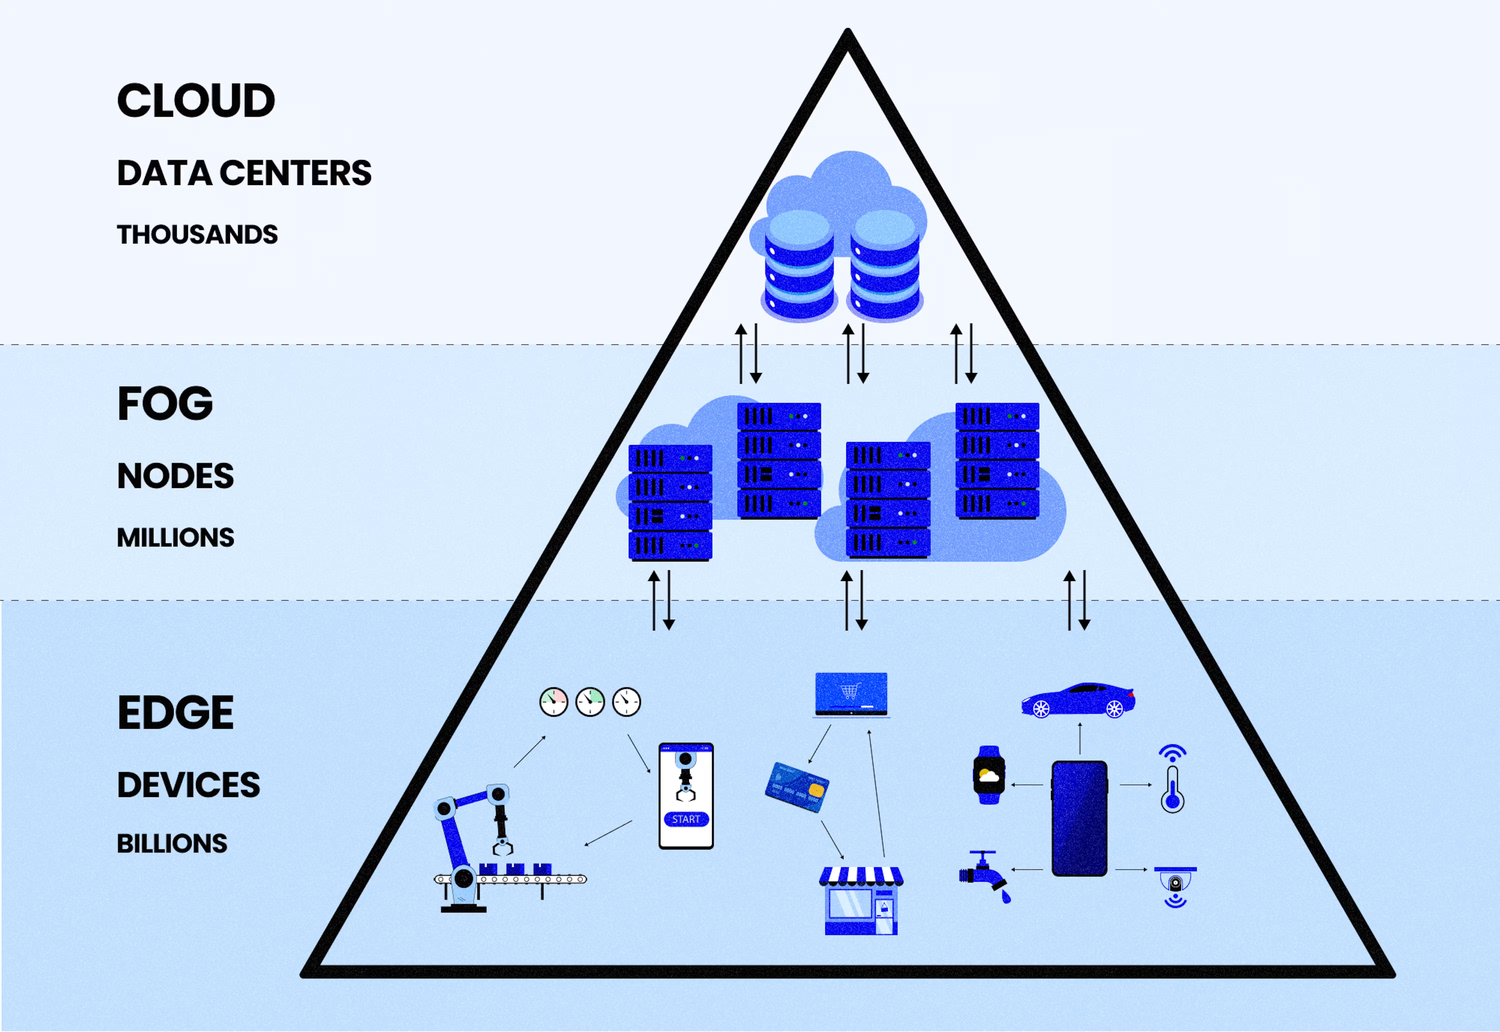
\includegraphics[width=0.5\textwidth]{report1_images/fog_edge1.png}
    \caption{Edge Computing Architecture and Data Processing Flow~\cite{maddevs_edge_computing}.}
    \label{fig:fog_edge}
\end{figure}

\noindent A real-world implementation that utilizes both paradigms is smart traffic management in intelligent transportation systems~\cite{ieee_vehicular_fog}. Vehicle sensors process 
immediate collision data locally at the edge devices, while local base station units operate as an intermediate fog layer nodes to coordinate traffic
flow and signal timings in real time.

\

% ==============================================================================
% SECTION: WEEK 2 - PROCESS: CONCEPT AND API
% ==============================================================================
\section{Week 2 - Process: Concept and API}

\subsection{Process Definition}

A process is essentially a program that being executed. When a process is running, the OS allocates
an address space in RAM (containing code, data, heap and stack) and the CPU read the instructions
and execute them on by one.

\hspace{5pt}

\noindent The differences between a process and a program lies in their execution state.
A program is stored as an executable binary on the disk, wheras a process is an active instance executing dynamically in memory.

\subsection{The Need for Processes}

Early computing executed single programs one at a time, which creates severe bottlenecks whenever a task had to wait for slow I/O operations, which forces the processor to idle. The 
abstraction of process was invented to solve this inefficiency, allows the OS to safely execute multiple programs concurrently with isolated memory.

\hspace{5pt}

\noindent The famous computer scientist Edsger W. Dijkstra has demonstrated the necessity of process through 
showing that breaking complex computing workloads into separated sequential execution units is essential to keep the CPU
continuously utilized while preventing tasks from overwriting shared data~\cite{dijkstra1968the}.

\subsection{Process Operations}

\subsubsection{Process Components}

A process comprises of four essential elements:
\begin{itemize}
    \item \textbf{Image of a program:} The compiled code, environment, and dependencies.
    \item \textbf{Memory (Address Space):} An isolated virtual address space allocated to each running process (shown in Figure~\ref{fig:process_address_space}). The program instructions data and static data remain fixed throughout execution, while two dynamic memory segments grow towards each other:
    \begin{figure}[H]
        \centering
        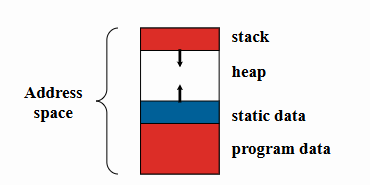
\includegraphics[width=0.40\textwidth]{report1_images/process1.png}
        \caption{Process Address Space Structure~\cite{cos40003_lecture2}.}
        \label{fig:process_address_space}
    \end{figure}
    \begin{itemize}
        \item \textbf{Stack:} Managed automatically by the CPU in Last-In, First-Out (LIFO) order to store variables, function parameters, and return addresses. It grows downward toward lower memory addresses.
        \item \textbf{Heap:} Managed at runtime for for dynamic memory allocation. It grows upward toward higher memory addresses.
    \end{itemize}
    \item \textbf{CPU state:} Registers, Program Counter (PC), and Stack Pointer (SP).
    \item \textbf{OS state:} Metadatas such as opened files, temporal statistics, etc.
\end{itemize}

\subsubsection{Context Switch}

\textbf{Context switch} is a mechanism that alternates the CPU between different processes to enable multitasking. Because a single CPU core can execute only one process at a time, the OS rapidly switches active execution contexts between processes (represented as programs \texttt{Prog1} and \texttt{Prog2} in Figure~\ref{fig:context_switch}) across four phases:
\begin{enumerate}
    \item \textbf{Phase 1 (\texttt{Prog1} Running):} \texttt{Prog1} executes instructions on the CPU, while \texttt{Prog2} remains suspended.
    \item \textbf{Phase 2 (Save State):} The OS saves the CPU registers, PC, SP of \texttt{Prog1}, placing it into suspension.
    \item \textbf{Phase 3 (Restore State):} The OS restores the previously saved registers, PC, and SP belonging to \texttt{Prog2}.
    \item \textbf{Phase 4 (\texttt{Prog2} Running):} \texttt{Prog2} takes over the CPU and resumes execution, while \texttt{Prog1} waits in memory.
\end{enumerate}

\begin{figure}[H]
    \centering
    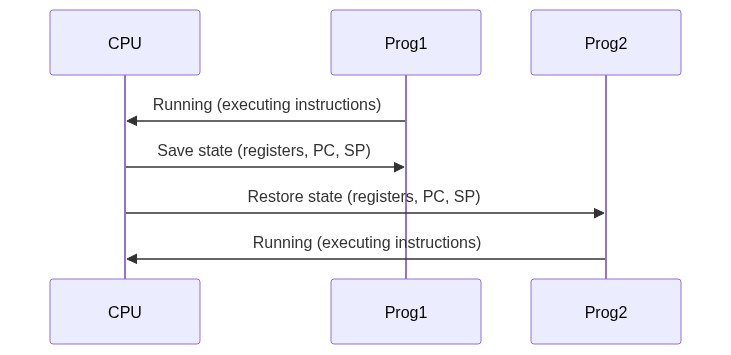
\includegraphics[width=0.62\textwidth]{report1_images/process2.png}
    \caption{Process Context Switching Mechanism Between Two Processes.}
    \label{fig:context_switch}
\end{figure}

\subsubsection{The Process Abstraction}

The \textbf{process abstraction} is a conceptual bridge between shared physical hardware and private program execution processes:
\begin{itemize}
    \item \textbf{Physical View:} One physical CPU shared and context-switched among processes.
    \item \textbf{Logical View:} Each process operates as if it has its own dedicated CPU and memory.
    \item \textbf{Time-Sharing:} Processes rapidly take turns using the CPU, enabling multi-computational processes on a single core.
\end{itemize}

\subsubsection{Process States}

A process transitions through three primary execution states:
\begin{itemize}
    \item \textbf{Ready:} The process is loaded in memory and prepared to run.
    \item \textbf{Running:} The process currently holds the CPU and is actively executing instructions.
    \item \textbf{Blocked:} The process has released control of the CPU to wait for an event (such as I/O completion) and cannot execute until that event happens.
\end{itemize}

\noindent Transitions between these states occur as follows:
\begin{itemize}
    \item \textbf{Ready $\rightarrow$ Running:} The scheduler picks the process to run.
    \item \textbf{Running $\rightarrow$ Ready:} The scheduler suspends the process.
    \item \textbf{Running $\rightarrow$ Blocked:} The process waits for an event (e.g., I/O request).
    \item \textbf{Blocked $\rightarrow$ Ready:} The event occurs (e.g., I/O completes).
\end{itemize}

\subsection{Process APIs}

There are three fundamental process management APIs in Unix systems.

\begin{enumerate}
    \item \textbf{\texttt{fork()} - Creating a Process by Duplication:} 
    
    Creates an exact clone of the caller with its own memory space. It returns \texttt{0} to the child process and the child's Process ID (PID) to the parent, allowing both to branch into different execution paths.
    
    \item \textbf{\texttt{wait()} - Synchronizing with Child Termination:} 
    
    Pauses the calling parent until one of its child processes finishes execution. It returns the terminated child's PID and collects its exit status, preventing zombie processes (dead processes waiting for their parents).
    
    \item \textbf{\texttt{exec()} - Replacing Current Program Code:} 
    
    Replaces the process's current memory contents (code, data, heap, stack) with a new executable program from disk. The process retains its original PID but executes the new code.
\end{enumerate}



% ==============================================================================
% REFERENCES
% ==============================================================================
\begin{thebibliography}{99}
\raggedright

\bibitem{pike2012}
R. Pike, ``Concurrency is not Parallelism,'' presented at \emph{Heroku Waza}, San Francisco, CA, USA, 2012. [Online]. Available: \url{https://go.dev/talks/2012/waza.slide#8}. 

\bibitem{techdifferences_concurrency_parallelism}
TechDifferences, ``Difference Between Concurrency and Parallelism,'' \emph{TechDifferences}, [Online]. Available: \url{https://techdifferences.com/difference-between-concurrency-and-parallelism.html}. 

\bibitem{rastergrid_simd_gpu}
D. Rákos, ``SIMD in the GPU world,'' \emph{RasterGrid Blog}, Feb. 2022. [Online]. Available: \url{https://www.rastergrid.com/blog/gpu-tech/2022/02/simd-in-the-gpu-world/}. 

\bibitem{gfg_distributed_system}
GeeksforGeeks, ``What is a Distributed System? Architecture and Components,'' \emph{GeeksforGeeks}, [Online]. Available: \url{https://www.geeksforgeeks.org/computer-networks/what-is-a-distributed-system/}. 

\bibitem{cern_wlcg}
CERN, ``The Worldwide LHC Computing Grid (WLCG),'' \emph{CERN}, [Online]. Available: \url{https://wlcg.web.cern.ch/}. 

\bibitem{wiki_cloud_computing}
Wikipedia, ``Cloud Computing,'' \emph{Wikimedia Commons}, [Online]. Available: \url{https://en.wikipedia.org/wiki/Cloud_computing#/media/File:Cloud_computing.svg}. [Accessed: Sep. 27, 2026].

\bibitem{ieee_vehicular_fog}
Z. Ning, J. Huang, and X. Wang, ``Vehicular Fog Computing: Enabling Real-Time Traffic Management for Smart Cities,'' \emph{IEEE Wireless Communications}, vol. 26, no. 1, pp. 87--93, Feb. 2019, doi: \url{https://doi.org/10.1109/MWC.2019.1700441}.

\bibitem{maddevs_edge_computing}
Mad Devs, ``Everything You Need to Know About Edge Computing,'' \emph{Mad Devs Blog}, [Online]. Available: \url{https://maddevs.io/blog/everything-you-need-to-know-about-edge-computing/}. [Accessed: Sep. 27, 2026].

\bibitem{cos40003_lecture2}
Swinburne University of Technology, ``Lecture 2: Process Concept and API,'' \emph{COS40003 Concurrent Programming}, 2026.

\bibitem{dijkstra1968the}
E. W. Dijkstra, ``The structure of the `THE'-multiprogramming system,'' \emph{Communications of the ACM}, vol. 11, no. 5, pp. 341--346, May 1968, doi: \url{https://doi.org/10.1145/363095.363143}.

\end{thebibliography}

\end{document}
